% -----------------------------------------------
% Template for ISMIR Papers
% 2016 version, based on previous ISMIR templates

% Requirements :
% * 6+1 page length maximum
% * 2MB maximum file size
% * Copyright note must appear in the bottom left corner of first page
% (see conference website for additional details)
% -----------------------------------------------

\documentclass{article}
\usepackage{ismir,amsmath,cite}
\usepackage{graphicx}
\usepackage{color}

% Title.
% ------
\title{word2vec applied to the Yale Corpus}

% Note: Please do NOT use \thanks or a \footnote in any of the author markup

% Single address
% To use with only one author or several with the same address
% ---------------
%\oneauthor
% {Names should be omitted for double-blind reviewing}
% {Affiliations should be omitted for double-blind reviewing}

% Two addresses
% --------------
%\twoauthors
%  {First author} {School \\ Department}
%  {Second author} {Company \\ Address}

%% To make customize author list in Creative Common license, uncomment and customize the next line
%  \def\authorname{First Author, Second Author}


% Three addresses
% --------------
\threeauthors
  {First Author} {Affiliation1 \\ {\tt author1@ismir.edu}}
  {Second Author} {\bf Retain these fake authors in\\\bf submission to preserve the formatting}
  {Third Author} {Affiliation3 \\ {\tt author3@ismir.edu}}

%% To make customize author list in Creative Common license, uncomment and customize the next line
%  \def\authorname{First Author, Second Author, Third Author}

% Four or more addresses
% OR alternative format for large number of co-authors
% ------------
%\multauthor
%{First author$^1$ \hspace{1cm} Second author$^1$ \hspace{1cm} Third author$^2$} { \bfseries{Fourth author$^3$ \hspace{1cm} Fifth author$^2$ \hspace{1cm} Sixth author$^1$}\\
%  $^1$ Department of Computer Science, University , Country\\
%$^2$ International Laboratories, City, Country\\
%$^3$  Company, Address\\
%{\tt\small CorrespondenceAuthor@ismir.edu, PossibleOtherAuthor@ismir.edu}
%}
%\def\authorname{First author, Second author, Third author, Fourth author, Fifth author, Sixth author}


\sloppy % please retain sloppy command for improved formatting

\begin{document}

%
\maketitle
%
\begin{abstract}
    We apply a word embedding model (word2vec) to a large corpus of classical music.
The first two principal components of the embeddings corresponding to major triads are arranged on the boundaries of a circular topology. In music from earlier composers, the topology is more well defined. Remarkably, the order in which major triads are arranged on this structure corresponds to their order in the circle of fifths. We situate our results in the context of current statistical research into functional harmony in common practice music. We then hypothesize reasons for the emergence of this structure.

\end{abstract}
%
\section{Introduction}\label{sec:introduction}

%!TEX root = ../ycac2vec.tex

\subsection{Word embeddings}
% lit review on word embeddings
Probabilistic models such as Latent Dirichlet Allocation \cite{Blei2003} are standard tools for analyzing text data. However, such models use bag-of-words representations. Therefore they extract meaning from word co-occurrance counts on the document level, and ignore the sequential nature of language. Syntax, punctuation, and grammar are intrinsically sequential, and a good model of natural language or tree structures should be able to capture both information from co-occurrance counts and information across time. While Latent Dirichlet Allocation has been used to model music (\textbf{Q:citation?}), music is inherently sequential. For in-depth analysis of style in music, we need embedding models.

Word embeddings, or real-valued vectors representing words in a vocabulary, were first introduced by \cite{Bengio2003} but popularized by \cite{Mikolov2013a}. Such models typically have a log-bilinear form \cite{Mnih2007}, and are trained using negative sampling with a fixed size context window \cite{Mikolov2013a}. This is equivalent to matrix factorization of a shifted pointwise mutual information word-context matrix \cite{Levy}. To see this, construct a co-occurrance matrix of words, where the rows and columns are the words in the vocabulary. Each entry $i, j$ in the matrix is the count of how many times word $i$ (e.g. `dog') ocurred in the context of word $j$ (e.g. `the'). Word embedding models such as the skip-gram model (word2vec) can be viewed as performing singular value decomposition on a transformed version of this matrix.  Compositional word embeddings for learning paragraph or document embeddings have also been proposed \cite{Le2014,Dai2015}. However, \cite{Levy2015a} suggests that much of the success of these types of distributed representations of words is due to the tricks needed to train such models such as noise contrastive estimation.


% lit review on word embeddings applied to things other than natural language
As useful models of discrete data, word embedding models are starting to be used in domains outside of natural language. For example, \cite{Asgari2015} embed protein sequences for classification, and \cite{Guardia-Sebaoun2015} develop an embedding model to build a recommendation system (for example, for recommending movies to users).
There exists some prior work on applying word embedding models to music. \cite{Name2015} trained an embedding model on a corpus of 200 rock songs for the task of recommendating chords to composers.

\subsection{Quantitative stylistic analysis of music}

\section{Methodology}\label{sec:methodology}

\subsection{Corpus}\label{corpus}

The Yale/Classical Archives Corpus (YCAC) is a database of pitch-class
and time data from MIDI files contributed by users of
classicalarchives.com encoding 8,980 distinct pieces of music
\cite{white2014yale}. Each piece is represented both by a sequence of
time-coded \texttt{music21.Chord} objects and additional local key estimations, which were obtained by ``salami slicing'' the original MIDI file. That is, a new chord token is created at every moment a voice enters or leaves the musical texture. To restrict the total vocabulary of the word embedding models to be applied later, we reduce each chord token to its chroma vector. A chroma vector is a twelve-place binary vector, one for each pitch-class. This choice also reflects the general programmatic interest of music theory in generalizing about rules of harmonic progression based on pitch content.\footnote{We discuss the possibilites of extending the present methodology to other important harmonic features (for example, pitch-class multisets or pitch sets) below}. 

A subset of the corpus was divided into four comparably-sized subcorpora based on the dates of composition of pieces, in fifty-year chunks from 1700--1899. Where an exact date of composition was not found in the piece metadata provided with the YCAC, the midpoint of the date range given in the metadata was used.\footnote{Typically, this range was the lifespan of the composer.}

\begin{table}
 \begin{center}
 \begin{tabular}{|l|l|l|}
  \hline
  Date range & No. pieces  & No. slices  \\
\hline
\hline
1700--1749 & 2 120 & 1 892 572 \\
\hline
1750--1799 & 1 806 & 2 820 522 \\
\hline
1800--1849 & 1 770 & 3 565 872 \\
\hline
1850--1899 & 1 601 & 2 635 754 \\
\hline

 \end{tabular}
\end{center}
 \caption{Piece (document) and slice (token) counts in the time-delimited subcorpora.}
 \label{tab:counts}
\end{table}

\subsection{Embedding space}\label{embedding-space}

A word2vec algorithm was used to train a number of word-embedding
spaces. First, a space was trained on the entire corpus to evaluate its plausibility. Then, four separate word-embedding spaces were trained on the date-delimited subcorpora described above. \footnote{The implementation used was the word2vec model provided by the Python module `gensim`, which uses a skip-gram negative sampling (SGNS) model which has been shown to be effective on large textual corpora. \cite{rehurek_lrec}}.
The algorithm treats each chroma vector as a word in a sentence. It
returns an n-dimensional real-valued vector for each word. t-SNE
dimensionality reduction was applied to the resultant word-embedding
space to demonstrate its plausbility. PCA was applied to the resultant
word-embedding space, and the locations of chroma vectors corresponding
to major triads were plotted.


\section{Discussion}\label{sec:discussion}

%!TEX root = ../ycac2vec.tex

As shown in Figure~\ref{fig:whole_corpus_circle_fifths}, we can see that the circle of fifths emerges from the structure of the learned vector space of chords in classical music.
This is not an intuitive result at first.
However, to see that this is a reasonable result of applying the skip-gram word2vec model, consider the log-likelihood of the model.
Gradients of the log-likelihood with respect to the embeddings are used to train the model.
The log-likelihood means the model will maximize the probability of correctly classifying the context given the training example.
If the model assigns too high a probability to correct contexts, it will be overconfident on other (incorrect) contexts, and the derivative of the log-likelihood will push the embeddings further apart.
But if the model assigns too low a probability to correct contexts, the gradient of the log-likelihood will flip signs and pull the embeddings closer together.
The minimal geometric structure that minimizes these constraints is a circle. If the parts of the circle are perturbed (e.g. imagine shifting the values of an embedding in the circle by a large amonut), the above arguments show that it will return to a circular structure by virtue of the gradients of the objective function.
We thus expect a circle from the principal components of highly stable embeddings (such as the embeddings of chords in the circle of fifths).
To see why the circle of fifths respects the ordering, we consider the context window (\textbf{(size 5? in our case)}).
Chords in the circle of fifths occur in each others' contexts, but usually only nearest neighbors (e.g. it is rare to see C major followed by B major).
Therefore C major and G major occur in each others' contexts and will be pushed closer together during training.
But they will be pushed apart from their non-nearest-neighbors (such as B major).
This shows they will respect the ordering apparent in classical music where common practices such as counterpoint result in transitions prevalent on the circle of fifths.


\section{Paper Length \& File Size}
Instead of the strict limit of six pages (last used in ISMIR 2014), we adopt
a ``(6+1)-page policy'' from ISMIR 2015 for ISMIR 2016. This means, the paper may have a
maximum of 6 pages for technical content including figures and possible references
with one additional optional 7th page containing only references.
Note that this is a strict requirement.
\textcolor{red}{The seventh page (if used at all) must
not contain any other material except for references.}

Paper should be submitted as PDFs and the \textcolor{red}{file size is limited to 2MB}. Please compress images and figures as necessary before submitting.

\section{Page Size}\label{sec:page_size}

The proceedings will be printed on
 \underline{portrait A4-size paper} \underline{(21.0cm x 29.7cm)}.
All material on each page should fit within a rectangle of 17.2cm x 25.2cm,
centered on the page, beginning 2.0cm
from the top of the page and ending with 2.5cm from the bottom.
The left and right margins should be 1.9cm.
The text should be in two 8.2cm columns with a 0.8cm gutter.
All text must be in a two-column format.
Text must be fully justified.

\section{Typeset Text}\label{sec:typeset_text}

\subsection{Normal or Body Text}\label{subsec:body}

Please use a 10pt (point) Times font. Sans-serif or non-proportional fonts
can be used only for special purposes, such as distinguishing source code text.

The first paragraph in each section should not be indented, but all other paragraphs should be.

\subsection{Title and Authors}

The title is 14pt Times, bold, caps, upper case, centered.
Authors' names are omitted when submitting for double-blind reviewing.
The following is for making a camera-ready version.
Authors' names are centered.
The lead author's name is to be listed first (left-most), and the co-authors' names after.
If the addresses for all authors are the same, include the address only once, centered.
If the authors have different addresses, put the addresses, evenly spaced, under each authors' name.
Here's a test of a citation. %\cite{jacoby_information_2015}

\subsection{First Page Copyright Notice}

Please include the copyright notice exactly as it appears here in the lower left-hand corner of the page.
It is set in 8pt Times.

\subsection{Page Numbering, Headers and Footers}

Do not include headers, footers or page numbers in your submission.
These will be added when the publications are assembled.

\section{First Level Headings}

First level headings are in Times 10pt bold,
centered with 1 line of space above the section head, and 1/2 space below it.
For a section header immediately followed by a subsection header, the space should be merged.

\subsection{Second Level Headings}

Second level headings are in Times 10pt bold, flush left,
with 1 line of space above the section head, and 1/2 space below it.
The first letter of each significant word is capitalized.

\subsubsection{Third and Further Level Headings}

Third level headings are in Times 10pt italic, flush left,
with 1/2 line of space above the section head, and 1/2 space below it.
The first letter of each significant word is capitalized.

Using more than three levels of headings is highly discouraged.

\section{Footnotes and Figures}

\subsection{Footnotes}

Indicate footnotes with a number in the text.\footnote{This is a footnote.}
Use 8pt type for footnotes. Place the footnotes at the bottom of the page on which they appear.
Precede the footnote with a 0.5pt horizontal rule.

\subsection{Figures, Tables and Captions}

All artwork must be centered, neat, clean, and legible.
All lines should be very dark for purposes of reproduction and art work should not be hand-drawn.
The proceedings are not in color, and therefore all figures must make sense in black-and-white form.
Figure and table numbers and captions always appear below the figure.
Leave 1 line space between the figure or table and the caption.
Each figure or table is numbered consecutively. Captions should be Times 10pt.
Place tables/figures in text as close to the reference as possible.
References to tables and figures should be capitalized, for example:
see \figref{fig:example} and \tabref{tab:example}.
Figures and tables may extend across both columns to a maximum width of 17.2cm.

\begin{table}
 \begin{center}
 \begin{tabular}{|l|l|}
  \hline
  String value & Numeric value \\
  \hline
  Hello ISMIR  & \conferenceyear \\
  \hline
 \end{tabular}
\end{center}
 \caption{Table captions should be placed below the table.}
 \label{tab:example}
\end{table}

\begin{figure}
 \centerline{\framebox{
 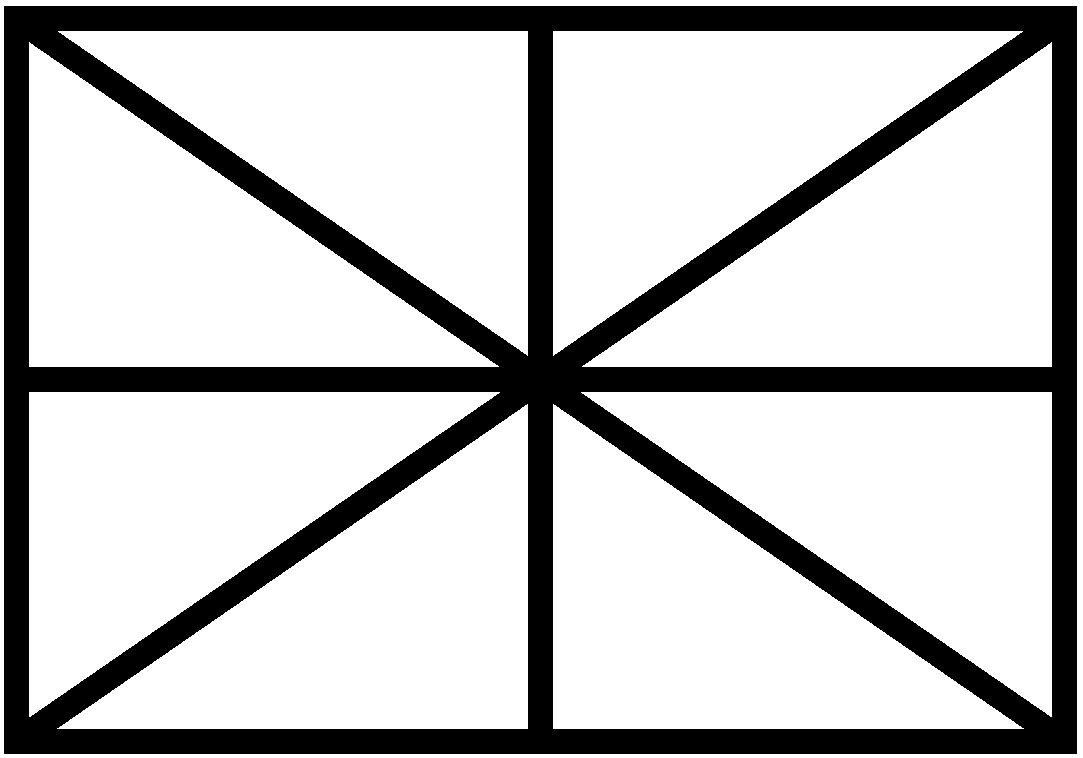
\includegraphics[width=\columnwidth]{figure.png}}}
 \caption{Figure captions should be placed below the figure.}
 \label{fig:example}
\end{figure}

\section{Citations}

All bibliographical references should be listed at the end,
inside a section named ``REFERENCES,'' numbered and in alphabetical order.
All references listed should be cited in the text.

\section{Acknowledgments}

The authors are grateful to Rajesh Ranganath for helpful discussions (and Dawen Liang? and anyone else who read the paper and gave feedback). Jaan Altosaar expresses gratitude to Prof. David Blei and the Natural Sciences and Engineering Research Council of Canada for research support.

% For bibtex users:
% \bibliography{ycac2vec}
\bibliography{/Users/jaanaltosaar/Dropbox/backups/mendeley_library/0music_mining.bib}

\end{document}
